% Main body with filler text
\section{PREDVAE}
\label{sec:methods}

% \subsection{Variational Autoencoders}
% \label{subsec:vae}

% A standard VAE, outlined in Fig. \textcolor{red}{[INSERT FIG]}, is composed of two neural networks referred to as the \textit{encoder} and the \textit{decoder}. The encoder is parameterized by $\boldsymbol{\theta}$ and maps an input vector $\mathbf{x}$ to a distribution over the lower-dimensional latent space, $q_{\boldsymbol{\theta}}(\mathbf{y}|\mathbf{x})$, where $\mathbf{y}$ denotes the latent space. The decoder is parameterized by $\boldsymbol{\phi}$ and takes as input samples $\mathbf{y}$ from the latent distribution. The aim of the decoder network is to learn a mapping from random samples of the latent space to the distribution over inputs, $p_{\boldsymbol{\phi}}(\mathbf{x}|\mathbf{y})$.

% \textcolor{red}{BLALBALBA SOMETHING SOMETHING ELBO AND VARIATIONAL INFERENCE.}

% The probabilistic nature of VAEs have proven to be a powerful tool for learning information-rich representations of inputs. The fact that distributions instead of point measures are learned allows for an expression of model uncertainty in the latent space. This feature means that VAEs are a viable tool for breaking degeneracies present in broad-band photometric observations lacking spectroscopic follow up, as is the case for photo-z estimation. \textcolor{red}{WRITE SOMETHING ABOUT THE DEGENERACY HERE, OR MENTION EARLIER?}

\subsection{Semi-Supervised Variational Autoencoders}
\label{subsec:ssvae}

\begin{figure}[ht!]
    \centering
    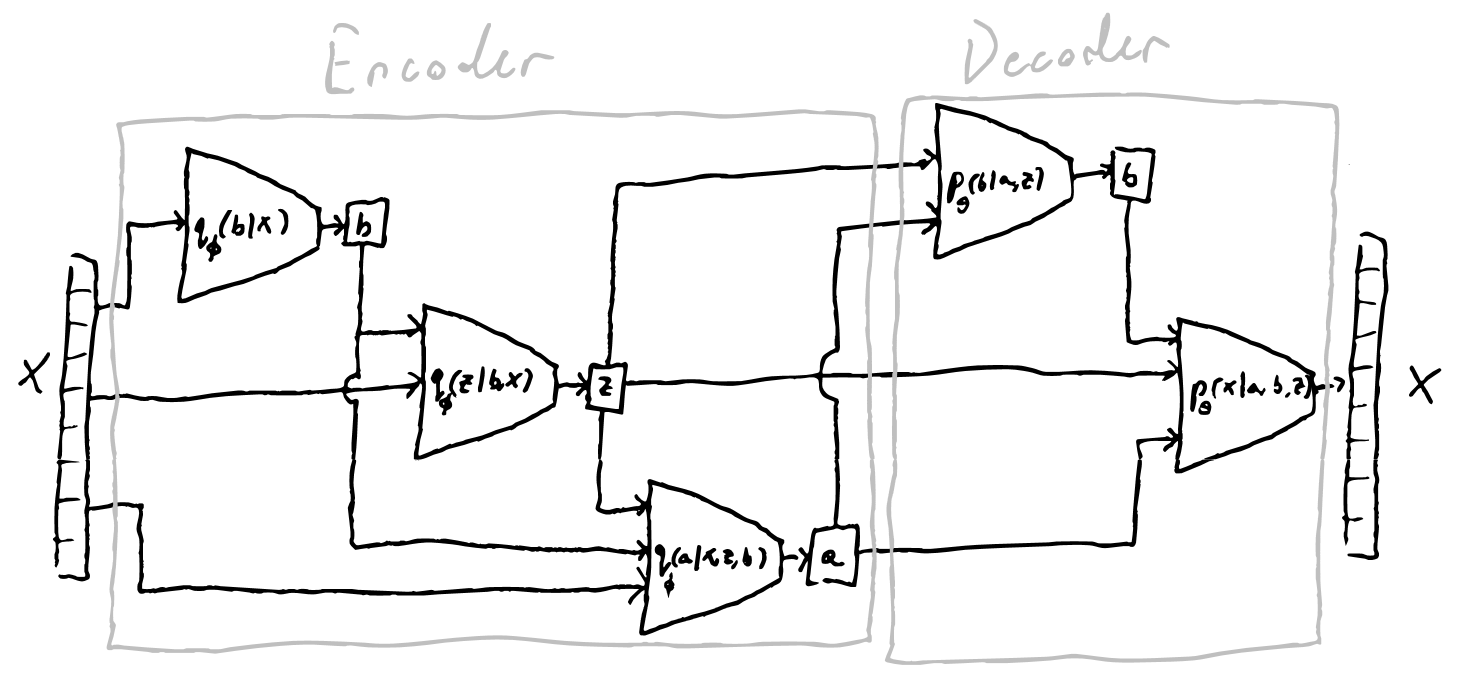
\includegraphics[width=\textwidth]{figures/model_sketch.png}
    \caption{Caption}
    \label{fig:sketch}
\end{figure}

Variational autoencoders (VAEs, first introduced by \cite{kingmaAutoEncodingVariationalBayes2022} and \cite{rezendeStochasticBackpropagationApproximate2014}, belong to a family of unsupervised neural networks that are trained to copy its input to its output in a probabilistic manner. This probabilistic mapping leads to a generative model that can be used to produce new samples from the input distribution. While VAEs have received attention in the past for their generative capabilities \textcolor{red}{[CITATIONS]}, their current utility stems from their ability to map a high-dimensional input into a lower dimensional compressed representation, known as the \textit{latent space}. In this setting VAEs have shown to be extremely competitive, being able to produce disentangled representations of complex inputs \textcolor{red}{[INSERT REPRESENTATION LEARNING PAPERS FROM LOCAL ZOTERO]}. 

Although VAEs have been applied to astrophysical use-cases before to disentangle data \textcolor{red}{[INSERT SOME OF THE ASTRO VAE PAPERS]}, they have seen little use in photo-z estimation. This is most likely due to the unsupervised nature of VAEs, which can only indirectly be applied to the case of photo-z estimation by using latent representations of photometric observations as training data for a supervised ML model. In such an approach there is no assurance that the latent representations are optimal for the secondary supervised learning task \citep{kingmaSemiSupervisedLearningDeep2014}. Extensive work has been done in extending VAEs to the semi-supervised setting, jointly learning disentangled representations \textit{and} classifications of data \textcolor{red}{[CITE KINGMA 14, MAALØE 16, OTHERS?]}.

In this work we make use of the approach outlined in \textcolor{red}{CITE MAALØE ET AL 16}, the general outline of which is shown in Fig. \textcolor{red}{INSERT SSVAE FIGURE}.


\subsection{Training}
\label{subsec:training}

hello world